%=========================
% Materials and Methods
%=========================
%============NOTE==============
% Check tense !!! It should be present and future tense and mostly passive voice.
%==============================

% 1. Why is this section in past tense? I thought when we talked in my office we agreed, Literature Review refers to work that's been done. Materials and methods refers to work that YOU want to do for your dissertation, which means it's not done yet unless this is your dissertation, in which case it's past tense because you're writing up what you've done for your research.

% Again. This "outline" seems to be a proposal. It should be written in FUTURE tense. You're writing this in a mishmash of present, future and mostly past tense. Save past tense for the dissertation after you've actually done the work.

This research will use data collected from surveys of irrigated lowland rice growing areas in South and South East Asia to examine relationships between the injuries caused by pests and diseases, cropping practices (e.g., rice variety grown, crop establishment method, fertilizer and chemicals applied), and rice yields. Their relationships will be constructed and analyzed through network analysis. I will develop and apply suitable methods of network analysis to characterize the associations of injuries and cropping practices. The resulting network of associations of injuries and cropping practices will thus provide a starting point for further investigations of their relationships (i.e., comparison of networks under different production environments or examination of networks at different levels of yield gains). 

Network analysis of rice crop health survey data is divided into three parts. In the following, I present three distinct network analysis approaches: single-network analysis, differential network analysis, and dynamic network analysis. These three approaches will answer different questions. I will apply single-network analysis to the data from all fields surveyed for identifying patterns of interactions between injuries and cropping practices and key components (e.g., most connected variables). Second, differential network analysis will aim to uncover similarities and differences of networks constructed from the different data sets (e.g., dry season versus wet season). Dynamic network analysis, the third type, will be applied to study how networks changed under at least two different aspects of an evolving complex system. Here, I will focus on dynamic networks by dividing farms into different levels of yield attained. 

\subsection*{Crop Health Survey Data}
\addcontentsline{toc}{chapter}{Crop health survey data}

%Rice is dominantly produced in Asia, 31 percent of the global rice harvested comes from Southeast Asia \shortcite{oecd2012oecd}. The highest levels of productivity are found in irrigated areas, where is the most intensified production system. Farmers can grow rice more than one crop per year here. Approximately 45 percent of the rice growing area in Southeast Asia is irrigated, with the largest areas being found in Indonesia, Viet Nam. Philippines and Thailand \shortcite{mutert2002developments}. In South Asia, major rice-growing countries are India and Bangladesh. India has the largest rice growing area (approximately 43 million hectares) in the world and contributes 25 percent of global rice production. 

% 1. You use survey and surveys twice in the first sentence. Of course it's survey data, you just said you used surveys. This doesn't flow. Reword.
% 2. Please use the proper title, this is a serious document.

Crop health survey data were collected through surveys of farmers' fields from 2009 to 2015 for both wet and dry seasons in different production environments across South and South East Asia representing irrigated lowland rice growing areas West Java, Indonesia; Mekong River Delta and Red River Delta, Vietnam; Tamil Nadu and Odisha, India; and Suphanburi, Thailand. The survey protocol described in the IRRI publication, ``A SURVEY PORTFOLIO TO CHARACTERIZE YIELD-REDUCING FACTORS IN RICE'', \shortcite{Savarysurvey2009} was used for data collection. The variables collected included environmental attributes, patterns of cropping practices, crop growth measurement and crop management status assessments, measurements of levels of injuries caused by pests, and direct measurements of actual yields from crop cuts. 

%The survey data described above consisted of measures of multiple variables. Theses variables were able to classify to three groups: cropping practices, injuries, and actual yield estimates. 

%\textbf{Injuries} were derived from time-dependent information on diseases, insects and weeds observed at four development stages of the growing crop: active tillering and active ripening. While injuries due to diseases and insects were specific to species (or species groups), information on weed infestation was the area covered by any weed species, either above or below the crop canopy. Information pertaining to injuries was collected in the form of number of injured organs (tillers, leaves and panicles), which later was made relative to the corresponding total number of organs present in the sampling units (12 hills per field for transplanted rice crops). As for weed infestation, the proportion of soil area covered at two levels of the crop canopy (below or above it) was assessed in three spots of 1 m\^{2} each. For this purpose, two types of injury indices were used: areas under injury progress curves or maximum level at any of the two observations, depending on the nature of the injury. The area under injury progress curve (AUIPC) was calculated by the mid- point method using the following equation:$ AUIPC = \sum \frac{1}{(x_{i} + X_{i-1})(T_{i} - T_{i-1})}$

%\textbf{cropping practices} included types of rice varieties, crop establishments, amount of fertilizers used, frequency of pesticides application. %\textbf{cropping practice set} was simplified, which collected with many type of data. For example, types of rice varieties (traditional varieties, modern varieties, and hybrid rice), crop establishments ( direct seeded, transplanted rice) were collected in categorical data, pesticide (molluscicide, herbicide, insecticide and fungicide) uses were collected discretized data, and accumulated organic, chemical fertilizers were collected in continuous data. \textbf{Injuries and diseases set} composed of specific signs caused by pests or pathogens (i.e., whitehead, brown spot). They were collected percent of incidence of injury at two rice stages (active tillering and active ripening stage). Two types of injury indices were used areas under progress curves or maximum level of injuries or disease incidence depending on the nature of the injury.

%The data that were collected at the individual field level were summarized in Table 1. These data were collected during four visits in each field during the rice growing season and described quantitative information on crop growth and levels of injuries to the crop due to pest (pathogens, insects and weeds) over time, as well as yield. Each field surveyed in each year was considered to be unique and was represented by a characteristic set of attributes pertaining to injuries and yield. 

%For this purpose, two types of injury indices were used: areas under injury progress curves or maximum level at any of the two observations, depending on the nature of the injury. The area under injury progress curve (AUIPC) was calculated by the mid- point method using the following equation:
%$ AUDIP = \sum \frac{1}{(x_{i} + X_{i-1})(T_{i} - T_{i-1})}$

%\begin{tubular}
%\hline
%Variable type & Variable & Variable description & unit \\
%\hline
%\end{tubular}

\section*{Single network analysis of crop health survey data}
\addcontentsline{toc}{chapter}{Single network analysis of crop health survey data}
\textbf{Introduction}

% Last sentence is unclear
Single-network analysis is used for analyzing a network based on a single data set. It aims to model patterns of relationships between entities to a network, thereby determining its topological properties such as node degree, degree distribution, average path length, clustering coefficient, modularity index \shortcite{newman2006modularity} to describe the patterns in the network model. These structural properties offer the potential to explore relationships within complex datasets. Additionally, it is used to identify keys drivers, which are key factors or clusters.

% These are only used for biological systems?
Correlation-based networks are applied to reveal the patterns of interactions or relationships of biological system. Their edges are obtained using correlation-based measures removing spurious relationships. Correlation based measures include linear based correlation (Pearson's correlation, partial correlation) and rank based correlation (Spearman's correlation, Kendall's correlation). Removal of spurious relationships is particularly important when one attempts to establish causal relationships between entities \shortcite{Toubiana:2013cv}.

In case of single network analysis, a cropping practices and injuries profiles network model based on whole data set of surveys. It was defined the correlation based network as undirected, weighted network. Nodes of the network corresponded to variables, and edges between variables were determined by the pairwise correlation.

%While this network was focused, it did not imply that only a single data set is used. Instead, appropriately similar multiple data sets can be used to validate the robustness of module definition and connectivity.
% objective

% 1. Isn't PCA and cluster analysis akin to correlation analysis? How are they the same? How is this different?
A network model based on crop health survey data has not yet been reported. Additionally, correlation analysis and network analysis of these data has not been studied. Thus, correlation measures and network approaches should be evaluated.

% what's the problem of multiple testing? Unclear.
According to \shortciteA{kolaczyk2014statistical}, correlation based network construction has at least three important issues to be dealt with. First, there is the choice of pair--wise correlation measure to be used. Second, the level of statistical significance must be determined for removal of sparse relationships. Finally, the problem of multiple testing must be considered because there are large numbers of tests for pair-wise comparison.

%An overview of cropping practices and injuries profiles network construction was depicted in Fig. 1: (a) data processing, (b) calculate correlation coefficients (Pearson, Spearman, or Kendall). Estimate \textit{p}-values for all coefficients. Next, determine threshold values for the resulting correlation coefficients will stored in adjacency matrices for the construction of networks, (c) Construct a network model, analyze network properties.

%The use of crop health survey data to construct co-occurrence network and perform network decomposition and network analysis has not yet been reported. Additionally, methods performing co-occurrence analysis and co-occurrence networks has not been studied. Thus, evaluation of such methods is challenging because there are many types of variables mixed in crop health survey data; methods can identify variables with true concordance often determine the prior knowledge; and methods performing biologically meaningful co-occurrence network construction. 

% methods

\textit{\textbf{Network construction}}

% 1. First sentence is unclear.
Cropping practices and injury profiles network are constructed by an adjacency matrix originating from the pair-wise correlations of the incidence of injuries (insect injuries and diseases), amount of fertilizer, the frequency of pesticide applied, type of rice varieties and crop establishment methods across different samples. Therefore, edges of the network correspond to the degree of correlation between two variables. A standard measurement of correlation between two variable $x$ and $y$, $cor(x,y)$, where WHAT??? has values between -1 to +1 depending on the level of relationships. $cor(x_{i}, x_{j})$ is equal -1 when there is a decreasing relationship between $x$ and $y$, and +1 when there is a increasing relationship.

To identify the most suitable pairwise correlation methods, I will evaluate four correlation based measures, Pearson's correlation, Spearman's rank correlation, Kendall's correlation, and biweight midcorrealtion. R was employed to compute pairwise correlation \shortcite{R:2014a}. The ``\texttt{cor.test()}'' function will be applied for generating a correlation matrix, which describes the pairwise correlations between variables. This function allows users to choose types of correlation measures to perform such as Pearson's correlation, Spearman's rank correlation and Kendall's rank correlation. To compute biweight midcorrelation, I will apply the ``\texttt{bicor()}'' function from the \textbf{WGCNA} package \shortcite{Langfelder:2008bd} in R. 

% 1. First sentence. Grammar and clarity.
% 2. Why would p-values be concerned? They aren't capable of such.
% 3. You need to revise this whole para for clarity.
% 4. Check your Bibliography, somethings not right with your R citation as it appears in the PDF.
When a correlation matrix is created, next is to construct the correlation based network from the resulting correlation matrix. However, \textit{p}-values should be concerned. As issues are mentioned above, \textit{p}-values must be adjusted for multiple testing. Benjamini-Hochberg adjustment or Bonferonni correction are recommended by \shortciteA{kolaczyk2014statistical}, which ``\texttt{p.adjust()}'' function in R can calculate adjusted \textit{p}-values. These values are compared to a standard 0.05 significance level. Correlation matrix contains pair-wise correlation coefficients, which have adjusted \textit{p}-values lower than 0.05 significant level. Alternatively, they are adjusted through control of the false discovery rate. The R package \textbf{fdrtool} can be implemented for this method \shortcite{fdrtool}.

% 1. First sentence, clarity.
% 2. Second sentence is not a sentence.
Up until this point, networks based on four association metrics (Pearson coefficient, and Spearman coefficient, Kendall coefficient and Biweight midcorrelation) will be constructed and assessed basic properties. I will apply R packages; \textbf{igraph} \shortcite{Csardi:2010wx}, \textbf{qgraph} \shortcite{qgraph}, \textbf{statnet}, \textbf{network} \shortcite{networkpackage} and \textbf{sna} to construct a network graph based on surveys, to decorate the network, and then analyze the network structure.

% 1. First sentence. Clarity/grammar
% 2. Second sentence. Clarity/grammar
A network modeled from biological data may not lead to reveal biological knowledge, even though it is created from a method based on its principle of statistical operation \shortcite{evaluationKumari}. For correlation based networks, edges correspond to correlation coefficients, and also affect to the network structure and behaviors. Different correlation based measures contribute to networks with different structures, even though they are constructed from the same data set. I will investigate the efficiency of networks based on four correlation measures for revealing the associations between variables of surveys. The most suitable correlation measure is assumed that it can contribute the network being able to reveal the associations between variables based on the existing literatures or good understandings of biological relationships between variables that crop health surveys observed.

%====================== Comments===================
% why knowledge of biological literature? Why not a good understanding of the biological system that you are monitoring? I think that's more essential and useful
% models cannot reveal knowledge, look up the definition of knowledge. It does not apply here. What do you really mean because it can not be knowledge?
% first sentence, all of them what?
% based on what study? Our study? Who is "we"? This is YOUR research. If anything it should be "based on my study" but I'm not clear as to what study you refer to here. Who are the "we" that are suggesting? You're the only author on this manuscript. It's your dissertation. There is no, our, us or we. It's only my, me, I here.
% Is "codes" the proper form to use?

\subsection*{Evaluating Network properties}

% 1. This whole para needs more information.
% 2. Your quotes are wrong here as they have been in several other places. I've corrected them in other spots for you several times. Please look up how to correctly use quotation marks in LaTeX.
Once a network is constructed, several indices can be computed to convey information about network structure. To evaluate the topological properties of both the interaction and the correlation based network, I will use the package \textbf{igraph} \shortcite{igraphpackage} \textbf{qgraph} \shortcite{qgraphpackage} in R. I particularly are interested in properties potentially relevant for biological roles and functioning as previously hypothesized in other biological networks \shortcite{ Strogatz:2001wc, qgraph, horvath2011weighted}.

\begin{enumerate}
\item Mean degree: the degree of a node counts the number of edges it has. The mean degree is calculated over all nodes in the network.
\item Degree distribution: the frequency of nodes vs. their (increasing) degree.
\item Average shortest path length: the shortest path between any two nodes is the single path with fewest edges between them. Alternative paths are feasible. The average shortest path length is the mean over all shortest paths between any two nodes in the network.
\item Mean clustering coefficient: a cluster of nodes is a triangle of nodes. The clustering coefficient calculates the fraction of observed vs. possible triangles for each node. The mean is subsequently determined from all nodes in the network.
\item Betweenness centrality: the betweenness centrality of a node is equal to the number of shortest paths between any two nodes in the graph passing through that node. The mean is calculated from all nodes in the network.
\item Closeness centrality: the closeness centrality of a node is given by the average distance of this node to any other node. Again, the network-wide measure is an average over all nodes in the network.
\end{enumerate}

\shortciteA{Deng:2012do, Toubiana:2013cv, horvath2011weighted, newman2003structure} are recommended references for descriptions of the network properties as well as the formal calculation of these measures.

%====================================================
\section*{Differential network analysis of crop heath survey data under different seasons and production environments}

% Should this analysis include more than one season or production environment since you say it's differential? Your section header above would indicate this to be true.

\addcontentsline{toc}{chapter}{Differential network analysis of crop health survey data under different season and production environment}

% introduction
% 1. First sentence. Grammar and punctuation.
% 2. Second sentence. Improper word usage.
Networks can response differently under various environments or with external signals. They can be more simplify by focusing on key components and capturing only the essential components differently responding between environments which they play a key role in the modeled response \shortcite{Peer:2011jd}. Networks are examined by adding or depleting some variables. This allows predicting interactions or components that change following the changed structure of networks. 

% 1. This para is difficult to understand. Revise.
Differential network analysis is applied to identify and describe differences between two networks under different conditions. Differential networks are created from different data sets or subtracted from one data set with different condition. Networks might display different interactions from the single network (from whole data set). The strongest interactions in differential networks are not necessarily that are strong in the single network. Conversely, the interactions are weak or removed from the differential network. If networks constructed from different environment conditions, the differential interactions between two networks are implied changes that they are a result of response to environmental conditions. Moreover, it can implied that environment conditions influence on the behaviors of pairs of nodes contributing to the differential interactions. 


% objective
% 1. Great first sentence!
% 2. Second sentence, however, needs work.
% 3. You change tenses in this para, you use three of them here.
The objective of differential network analysis is to extract interactions from the original network that appear to be active under different conditions. I focus on two aspects of this analysis. The first is to compare how patterns of interactions of cropping practices and injury profile network changed across multiple production environments. The second is to study how networks changed under different seasons. Each data sets is then used to construct the network. Next, these networks are contrasted to find a) non-preserved modules, b) differentially occurred variables, and c) differentially connected variables.
% methods

% 1. Last sentence is awkward.
Based on the methods of single network construction mentioned above, differential networks were constructed from the survey data with different groups of samples following the purpose of network construction. To analyze differential networks under different seasons, I will construct two networks; one will be constructed from dry season data, and another will be constructed from wet season data. Additionally I will determine differential networks under different production environments (locations).
.

% 1. You applied the package or a function from a package? # I do not know excectly what function I will use, so I stated the packages that I will use instead of functions of those packages.
For comparison with a standard differential network analysis, I applied \textbf{WGCNA} \shortcite{horvath2011weighted} and \textbf{dna} \shortcite{dnapackage} package in R, which this package provide several function to analyze the differences of topologies of two networks \shortcite{horvath2011weighted}. 


These packages includes preprocessing tools for simultaneously preparing a pair of networks for analysis, procedures for computing connectivity scores between pairs of variables based on many available statistical techniques, and tools for handling modules of variables based on these scores. Also, procedures are provided for performing permutation tests based on these scores to determine if the connectivity of variables differs between the two networks, to determine if the connectivity of a particular set of important variables differs between the two networks, and to determine if the overall module structure differs between the two networks. Several built-in options are available for the types of scores and distances used in the testing procedures, and additionally, the procedures provide flexible methods that allow the user to define custom scores and distances. For example,``\texttt{test.modular.structure()}'' function is used to compare between the connectivity measures of each network \shortcite{dnapackage}. 

%I propose the overview of differential networks are illustrated in Figure \ref{fig:wholenet}.


% why is 2.3 not 2.1? % The problem there is that you must put the label after a caption, so the label can reference to the figure (it references to the caption, actually). See here: http://www.latex-community.org/forum/viewtopic.php?t=3659 I've corrected this. - ahs
 

\section*{Dynamic network analysis of crop health survey data}
\addcontentsline{toc}{chapter}{Dynamic network analysis of crop health survey data} % okay edit one more round for more consistency
% introduction
Networks can dynamically respond and adapt to the internal state and external signals \shortcite{Peer:2011jd}. As the internal state, backgrounds of nodes influence the structure and behavior of the network and give rise to significant differences across individuals. Backgrounds are included information about where the data are from. The different sources and different times collecting the data strongly determine the network behaviors. 

% 1. First sentence, unclear, revise.
% 2. Sentence that starts, "It seems clear" is unclear. Revise.
% 3. Revise last sentence for flow.

Biological systems are highly dynamic. They must continuously respond to a external signals or internal state of the system. The responses can be altered slowly or fast over time \shortcite{Peer:2011jd}. Thus, realistically the corresponding biological networks evolve as well, and should be analyzed.  It seems clear that if we are able to construct the dynamic networks that enable to see and understand the systems on how their dynamic effects are changed overtime, we will understand biological systems. Some understandings were obtained from studies of dynamics of large networks, for example, gene expression or metabolic fluxes network \shortcite{Idekerdiffnet}.
 
% 1. Revise first sentence for flow.
% 2. Second sentence. Revise for spelling and clarity.
% 2. Third sentence. Revise for spelling and clarity.
Dynamic network analysis is applied for study changes of networks at least two different aspects of an evolving complex system. 

The main goal of dynamic network analysis moves away from single network analysis, which characterizes absolute properties of the system. It aims to concentrate on a specific dynamic systems response. Rather than answer what the key factors in the system, they answer what parts of the system are most affected by perturbation. Most commonly, dynamic networks are applied when the edges among a set of vertices or the sets of vertices itself are changing as a function of time. However, in the context of crop health surveys, I will apply dynamic networks to capture the yield-varying behaviors through different survey datasets are grouped by different levels of yield measurements.

% 1. First sentence. Revise wording.
% 2. Second sentence. Revise for flow and wording.
% 3. Third sentence, capitalization.
% 4. Third sentence, flow.
% 5. Fourth sentence, where is the rest of it?
%From the previous study of \shortciteA{Savary:2000vr}, levels of actual yields are affected by different patterns of interactions between injuries and cropping practices. The results from damages of pests and disease affect to yield loss. Hypothetically, different yield gains are the consequence of different patterns of interaction between injuries and disease, and production situations.  From the context of crop health survey data, 

% 1. Different means there is a difference. Your first sentence only contains one level, how can it be different?
% 2. Second sentence, incomprehensible.
% 3. Third sentence. Revise for flow.
My objectives are to construct and analyze networks of crop health survey data at different levels of farmers' yields. Surveys contained records of estimated actual yields, various types of injuries and cropping practice. To obtain the data for constructing the dynamic network, I will group the data with successive levels of the yields, and obtain different yield data set in order to construct a dynamic network of yield-varying behaviors. I then will employ \textbf{networkDynamic} \shortcite{networkdynamicpackage} and \textbf{ndtv} \shortcite{ndtvpackage} packages to generate yield-varying networks. The dynamic graphs will be characterized following \shortcite{bilgin2006dynamic, kolaczyk2014statistical}. From the network based perspectives, the results will show the patterns of interactions between nodes how they changed when levels of yield decreased or increased.

%\begin{landscape}

%\begin{figure}[h!]
%\centering
%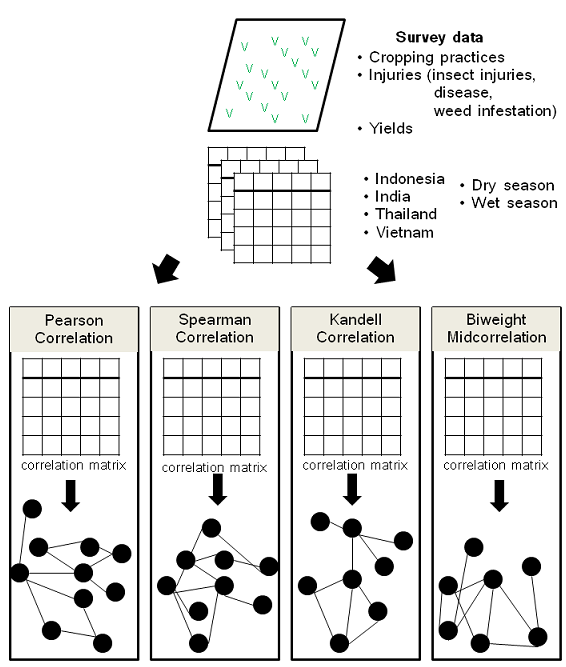
\includegraphics[resolution = 600]{pipeline}
%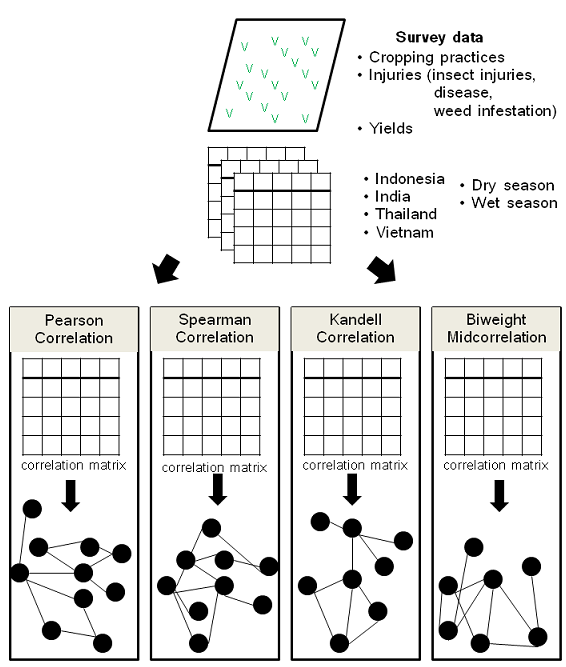
\includegraphics[width=6in]{pipeline}

%\caption[Proposed pipeline for network construction]{Proposed pipeline for network construction. (a) Collect the input profiling data and output profiling data from different samples and different locations. (b) Calculate correlation coefficients (Pearson, Spearman, or Kendall). Estimate P-values for all coefficients. Next, determine threshold values for the resulting correlation coefficients and \textit{P} values, storing results in adjacency matrices for the construction of networks. (c) Construct network and analyze network for graph-theoretic properties and infer biological meanings and integrate the network of input data and output data. (d) Repeat analysis for a second season to verify the network model.}
%\label{fig:pipeline}
%\end{figure}
%\end{landscape}

%\newpage
%\begin{landscape}
%\begin{figure}[h!]
%\centering
%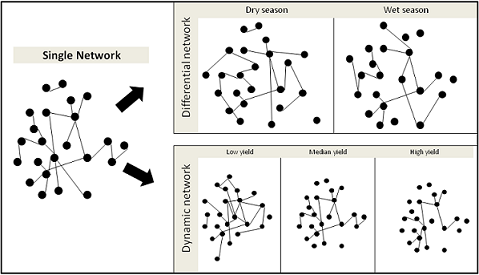
\includegraphics[width=6in]{wholenet}

%\caption[Network comparison]{Network comparison: Network models constructed from survey datasets of different geographic locations are compared by determining their properties. Networks will express the conserved domains within their structure. A merged representation of the two networks being compared is also proposed as a holistic network of rice ecosystem in South and South East Asia.}
%\label{fig:wholenet}
%\end{figure}
%\end{landscape}

%================eos================================